w%% A simple template for a lab or course report using the Hagenberg setup
%% with the standard LaTeX 'report' class
%% äöüÄÖÜß  <-- keine deutschen Umlaute hier? UTF-faehigen Editor verwenden!

\documentclass[a4paper,english,11pt]{report}		
%\documentclass[a4paper,ngerman,11pt]{report}

\usepackage{hgb}
\usepackage{hgbabbrev}
\usepackage{hgblistings}
\usepackage{hgbbib}
\usepackage{hgbheadings}

\RequirePackage[utf8]{inputenc}		% remove when using lualatex oder xelatex!

\graphicspath{{images/}}  % where are the images?
\bibliography{literatur}  % requires file 'literatur.bib'

\author{Sascha Zarhuber\\ S1510629021}
\title{IM690\\ \emph{Event-based build pipeline for static content management}\\ Project Report}
\date{\today}

%%%----------------------------------------------------------
\begin{document}
%%%----------------------------------------------------------
\maketitle
\tableofcontents
%%%----------------------------------------------------------

\chapter*{Abstract} % Vorwort

With a constantly growing number of internet users worldwide, websites are facing a difficult challenge nowadays: Serving information \emph{without delay}.

Static site generators build websites which don\textquotesingle t need to interfere with any other service when requested by a client, and are therefore saving precious time and resources, if configured properly. A big drawback however is the amount of \textbf{time}, \textbf{configuration} and \textbf{resources} needed for rebuilding the website every time its content changes.

This project should reveal possibilities to overcome these challenges, mainly using a \emph{selective approach} to only render parts which have changed, but also are crucial to the project\textquotesingle s contents.


%%%----------------------------------------------------------
\chapter{Initial situation}
%%%----------------------------------------------------------

Static site generators are growing fast and are more and more used as a replacement for common content management systems.

The main advantage are their independence of \emph{external} services, like database systems, session caching services, etc\ldots\newline Also, they seldomly consist of complicated backend systems and are mostly created in pure \textbf{HTML} or simple markup languages like \textbf{Markdown}.\footnote{Markdown: \url{https://daringfireball.net/projects/markdown/}}
%
\begin{figure}[p]
    \centering
    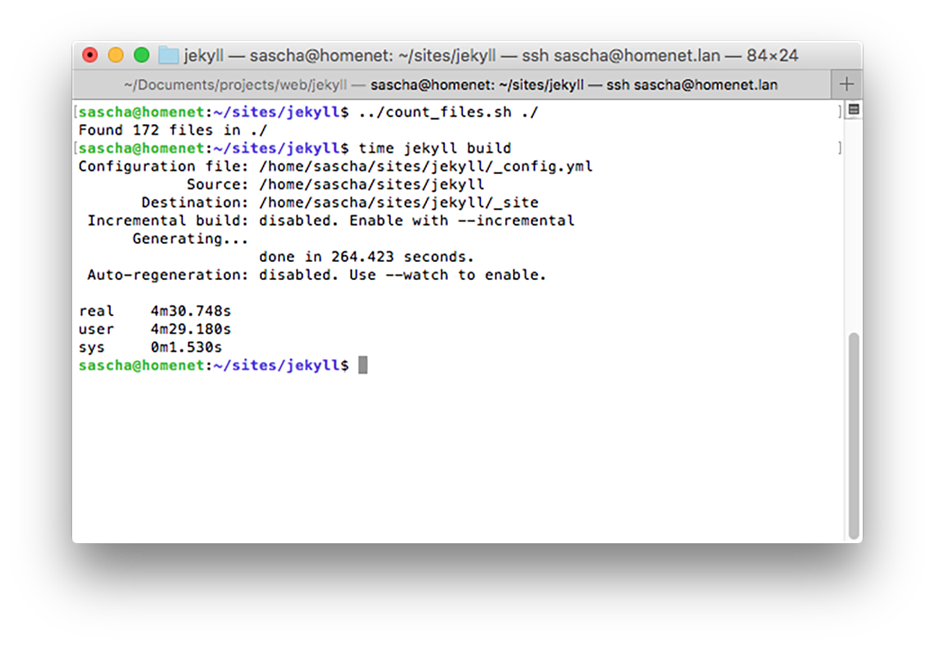
\includegraphics[width=0.8\textwidth]{jekyll_build.png}
    \caption{A screenshot showing the build time for the webroot of\newline \url{https://jekyllrb.com}. 172 files were generated in approximately 4:30 minutes.\\ The result is a complete webroot containing browser readable \emph{HTML} pages, assets, style sheets and \emph{JavaScript} files.}
    \label{fig:jekyll_build}
\end{figure}
%

One of the biggest drawbacks however, is the fact, that static site generators have to preprocess every bit of information they contain (\emph{see Fig. \ref{fig:jekyll_build}}). This is the complete opposite compared to other content management systems, which process information \emph{on request}. This means, that user-readable content is fetched and rendered \emph{just in time} it was requested from the client.

Therefore, depending on the setup, a dynamically growing amount of time needed for a build cycle might be the case.
For being able to work against this fact, a working approach has to be found, which saves time by \emph{leaving out} information, which has not changed since the previous build.
%

%%%----------------------------------------------------------
\chapter{Implementation}
%%%----------------------------------------------------------

%
\begin{figure}[p]
    \centering
    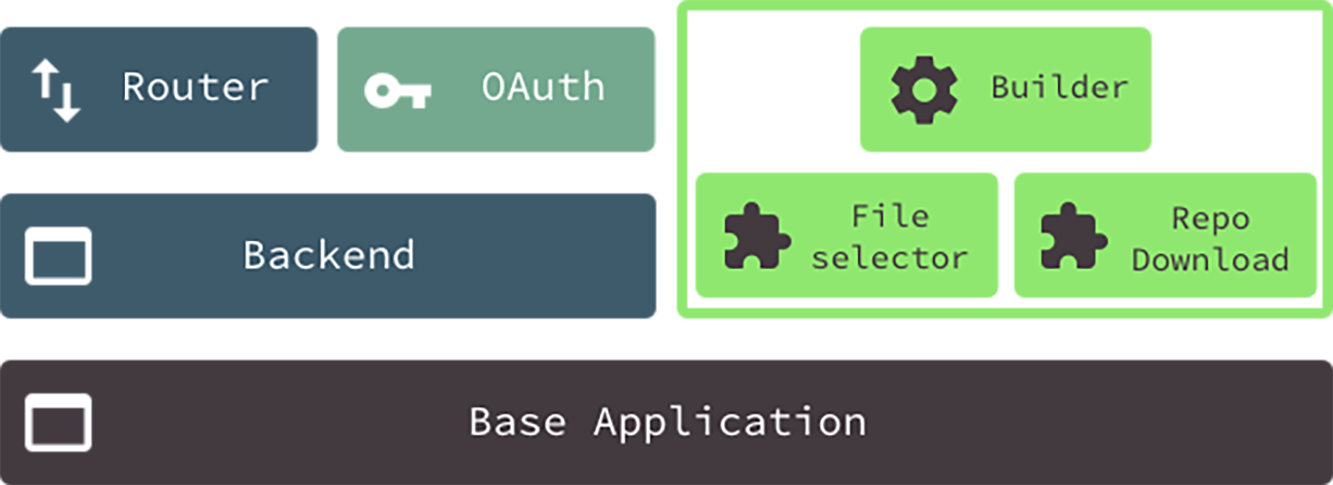
\includegraphics[width=0.9\textwidth]{application_structure.png}
    \caption{A graphic showing the base structure of the implemented application.\\ The \emph{base application} layer serves as foundation, containing necessary libraries for implementing the \emph{HTTP} specifications. The \emph{routing} and \emph{OAuth} layer are responsible for authenticated requests to the endpoints, whilst the \emph{builder package} is designed as a partly autonomous, loosely coupled rendering service.}
    \label{fig:application_structure}
\end{figure}
%

The project itself was intended to work as a stand-alone service, thus leading to the advantage of not having to install a complete project setup locally on the \emph{content producer} side. Additionally, one of the first design decisions was to closely couple this project with the \emph{GitHub API}\footnote{GitHub API: \url{https://developer.github.com/v3/}}.

Both of these decisions should lead to a fully customizable production environment, easy to setup and adapted to each desired workflow, without having the need of making a compromise prior to getting workload done.

\section{Framework choice}
Although there are a lot of static site generator frameworks available, I mainly concentrated on comparing the following two, before setting up my project application:

\subsection{Jekyll}
\textbf{Jekyll}\footnote{Jekyll: \url{https://jekyllrb.com}} --- the leading static site generator with more than 28,000 stars on \emph{GitHub}\footnote{Jekyll repository on GitHub: \url{https://github.com/jekyll/jekyll}}, was responsible for a renaissance of statically generated websites, when it was introduced in 2008\footnote{Jekyll history: \url{https://jekyllrb.com/docs/history/}}.\newline Originally introduced by \emph{Tom Preston-Werner}, one of the co-founders of \emph{GitHub}, it quickly grew a big community around it, benefitted mostly due to its wide usage on \emph{GitHub pages}\footnote{GitHub pages: \url{https://pages.github.com}}.

However, \emph{Jekyll} is written in \textbf{Ruby}, which causes a bit of friction, when trying to embed it into a server-side \emph{JavaScript}-based ecosystem. Another huge disadvantage might be, that this framework is one of the most opinionated to my knowledge. As an example, a typical \emph{Jekyll} project bootstraps as follows:

\begin{itemize}
\item Uses Shopify\textquotesingle s \emph{Liquid} templating system, strongly coupled to the project\textquotesingle s variable structure
\item References pre-built \emph{Ruby} gems, even for \emph{SEO}-specific definitions
\item Includes already a \emph{Sass}-setup right from the start
\item Might fail to produce output because of unsupported versions of referenced \emph{Ruby} gems (\emph{see Fig. \ref{fig:jekyll_fail}})
\end{itemize}

%
\begin{figure}[p]
    \centering
    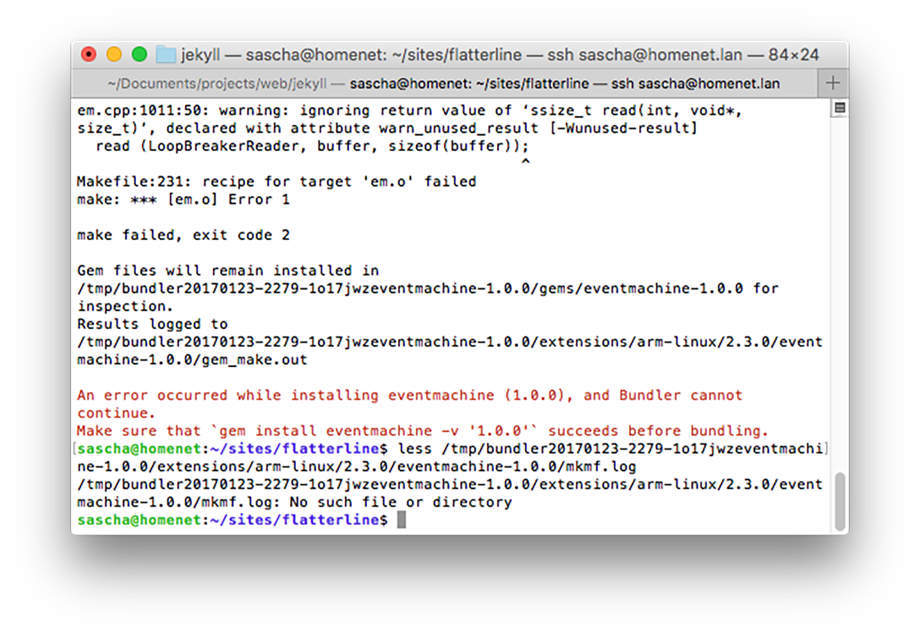
\includegraphics[width=0.8\textwidth]{jekyll_fail.png}
    \caption{A screenshot showing a failing \emph{Jekyll} build due to mismatching versions of a certain \emph{Ruby} gem.}
    \label{fig:jekyll_fail}
\end{figure}
%

\subsection{Metalsmith}
\textbf{Metalsmith}\footnote{Metalsmith: \url{http://www.metalsmith.io}} --- a very modular static site generator on the other hand, is completely written in \textbf{JavaScript}, which makes it easier to integrate it into \emph{Node.js}-based applications. Furthermore, it consists basically just of modules, so that every job inside the build pipeline gets handled from its own module. The whole application may be put together and extended like using \emph{LEGO} bricks.

Due to the possibility of heavily customizing a \emph{Metalsmith} setup to your needs, the decision was made in favor of this framework, although a few challenges remained:

\begin{itemize}
\item A working remap of \emph{Jekyll\textquotesingle s} variable structure to \emph{Metalsmith} could not be realized. Both projects handle their build cycles too different. This makes it even harder to compare my intended selective approach to conventional \emph{Jekyll} project setups.
\item Shopify\textquotesingle s \emph{Liquid} template engine has not been fully ported to \emph{JavaScript} till this day. It easily breaks when using custom functionality within template files.
\item Custom project setups in general require a customized, adaptive handling during build time. This concerns not only \emph{Jekyll} projects, but also customized \emph{Metalsmith} projects.
\end{itemize}

\section{Application structure}
The application itself was bootstrapped from an \emph{Express.js}\footnote{Express.js: \url{https://expressjs.com}} base configuration. To persist user, project and build information, the online \emph{MongoDB}-service \emph{mLab}\footnote{mLab: \url{https://mlab.com}} was used, as it provides a free tier for testing purposes. 

Using this persistence possibility, an additional authentication service was realized using \emph{OAuth2orize}\footnote{OAuth2orize: \url{https://github.com/jaredhanson/oauth2orize}}. This makes it easier to provide an application-wide user management system, which does not require any \emph{HTML} login form.

In the end, the application featured a routing service to different API-endpoints, an \emph{OAuth2.0}-authentication service and a decoupled building service containing access to the \emph{GitHub API}, as well as a very basic \emph{Metalsmith} setup (\emph{see Fig. \ref{fig:application_structure}}).

%
\begin{figure}[p]
    \centering
    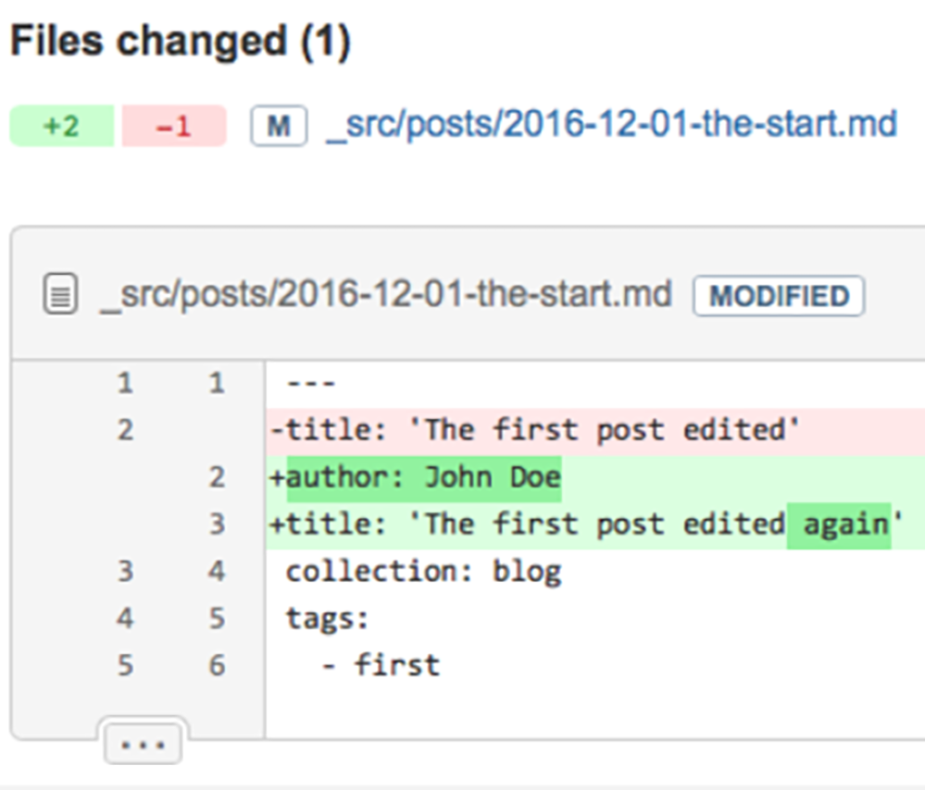
\includegraphics[width=0.65\textwidth]{diff_sample.png}
    \caption{A screenshot showing a \emph{diff} of two different revisions of a file. In this case, the \textbf{author} information was added above the \textbf{title} field, compared to the previous version. Furthermore, the term ``again'' was also added to the \textbf{title} string.\\ Overall, this file features 2 additions and 1 deletion.}
    \label{fig:diff_sample}
\end{figure}
%
\section{Selective approach}
To get a basic overview on which parts have changed, a file comparison using \textbf{diff} is very supportive in this case. Not only does it show how different files have been altered (\emph{added}, \emph{modified} or \emph{deleted}), but also which contents faced a change (\emph{see Fig. \ref{fig:diff_sample}}).

To compare the actual state of the project, the current project branch has to be checked out. Furthermore a \emph{diff} between the latest build state as \emph{base}-reference and the current \emph{HEAD}-reference shows the file changes within the given project. A sample request for such a \emph{diff} would be for example:
\begin{center}
\url{https://github.com/saschazar21/twitter-infovis/compare/777f148...b3c84ab.diff}
\end{center}

The above URL shows a raw \emph{diff} of a sample repository between commits \textbf{777f148} as \emph{base} and \textbf{b384ab} as \emph{head} for all files involved. Due to the fact, that this is basically only a simple output from a console program, this functionality would later be not anymore limited to \emph{GitHub} alone.

Being able to investigate the altered contents of the project using \emph{diff}, it now only needs to temporarily delete all unmentioned files from the source directory before performing a build. After a successful build though, the contents of the newly rendered remaining files in the source need to be merged with the previous state of the project to form a complete website in the end.

%%%----------------------------------------------------------
\chapter{Milestones acquired}
%%%----------------------------------------------------------

\begin{itemize}
\item GitHub API integration
\item Provide ecosystem for web project builds
\item Compare states using diff
\item Keep track on build states
\item Create a possible testbed for render measurements
\end{itemize}



%%%----------------------------------------------------------     
\chapter{Intended project goals}
%%%----------------------------------------------------------

\begin{itemize}
\item Render or re-render static webroots seamlessly
\item Provide latest build as archive for deployment
\item Make service responsive to GitHub webhooks
\item Integrate into CI services
\end{itemize}


%%%----------------------------------------------------------
%\MakeBibliography[nosplit]
%%%----------------------------------------------------------

\end{document}
